\chapter{Introdução}
\label{cap:introducao}

%Para começar a usar este \textit{template}, na plataforma \textit{ShareLatex}, vá nas opções (três barras vermelhas horizontais) no canto esquerdo superior da tela e clique em "Copiar Projeto" e dê um novo nome para o projeto. 

% Para começar a utilizar este \textit{template}, siga o tutorial clicando no seguinte \textit{link}:
% \url{https://biblioteca.ufc.br/wp-content/uploads/2015/09/tutorial-sharelatex.pdf}

% Neste \textit{template}, o autor irá encontrar diversas instruções e exemplos dos recursos do uso do \LaTeX~na plataforma \textit{Overleaf}. O \LaTeX~foi desenvolvido, inicialmente, na década de 80, por Leslie Lamport e é utilizado amplamente na produção de textos matemáticos e científicos, devido a sua alta qualidade tipográfica \cite{goossens1994latex}.

% O \textit{ShareLatex} é uma plataforma \textit{online} que pode ser acessado por meio de qualquer navegador de internet até mesmo de um \textit{smartphone}. Essa plataforma dispensa a instalação de aplicativos no computador para desenvolver trabalhos em \LaTeX. Também, não é necessário instalar \textit{packages}, ou seja, pacotes que permitem diferentes efeitos na formatação e no visual do trabalho. Todos os \textit{packages} que este \textit{template} utiliza são encontrados \textit{online}.

% Apresentam-se, também, neste modelo, algumas orientações de como desenvolver um trabalho acadêmico. Entretanto, este arquivo deve ser editado pelo autor de acordo com o seu trabalho sendo que a formatação já está de acordo com o aceito pela Universidade Federal do Ceará.  

% A introdução, tem como finalidade, dar ao leitor uma visão concisa do tema investigado, ressaltando-se o assunto de forma delimitada, ou seja, enquadrando-o sob a perspectiva de uma área do conhecimento, de forma que fique evidente sobre o que se está investigando; a justificativa da escolha do tema; os objetivos do trabalho; o objeto de pesquisa que será investigado. Observe que não se divide a introdução em seções, mas a mesma informa como o trabalho ao todo está organizado.



% Inicio -------------------------------------------

\section{Motivação}\label{sec:Motivacao}

Doenças cardiovasculares \gls{DCVs} são a principal causa de morte em todo o mundo, representando aproximadamente 17,9 milhões de mortes por ano, o que corresponde a 31\% de todas as mortes globais como mostra a pesquisa \cite{who2021cardiovascular}. Dentre as DCVs, as arritmias cardíacas são condições comuns que podem levar a eventos adversos graves, como parada cardíaca súbita. A detecção precoce e precisa de arritmias é crucial para a prevenção de complicações e melhoria dos resultados clínicos. Segundo o jornal USP doenças cardiovasculares são a principal causa de morte no Brasil, representando cerca de 30\% de todas as mortes no país \cite{jornalusp2024doencas}.

Este trabalho trata de dados de pacientes que ficaram em observações clínicas e acompanhamento que apresentaram sitomas de arritmia cardíaca, esses dados foram coletados pela plataforma PhysioNet \cite{physionet2020music}. Em resumo a população do estudo é de 992 pacientes com insuficiência carciaca crônica \gls{ICC} esses dados de coletas trata do ano entre abril de 2003 e dezembro de 2004, com um acompanhamento de uma mediana de 44 meses até 2008 de dezembro, alguns desses
pacientes apresentaram eventos de morte súbita cardíaca \gls{MSC}, as coletas foram feitas em 8 hospitais universitários espanhóis, na Espanha pela cidades de Barcelona, Sevilha, Cádiz, Múrcia, Santiago de Compostela, esses conjunto de dados de sinais e a organização desse banco de dados que foi parar no PhysioNet foi liderada pelo Instituto de Investigación de Ingeniería de Aragón \gls{I3A} \cite{physionet2020music}, na Universidade de Zaragoza (Zaragoza, Espanha), pelo grupo do pesquisador Pablo Laguna.



\section{Base de dados}\label{sec:BaseDeDados}

De acordo com a pesquisa \cite{physionet2020music}, os dados coletados incluem sinais de ECG Holter de 24 horas de 3 derivações (96\%) e 2 derivações (4\%), dados de eletrocardiograma \gls{ECG} em repouso de alta resolução com três derivações de 20 minutos, além de dados clínicos e demográficos dos pacientes, ecocardiografia e exames laboratoriais de sangue. Esses dados foram registrados em uma tabela CSV com 105 variáveis. Os dados são ricos tanto em sinais de ECG para o encontro de padrões de ondas e intervalos, como o QT, mudanças nas frequências, amplitude de onda e picos RR, quanto em dados clínicos e demográficos, o que permite uma análise abrangente dos fatores de risco associados a eventos cardíacos adversos. Existem vários métodos para análise usando esses dados; dentre as variáveis citadas, existe duas variáveis que irei usar como ponto de partida que se chama Follow-up period from enrollment (days)  \cite{physionet2020music_dataset}. Que se trata o tempo do período de acompanhamento dos pacientes, ou seja, o tempo que os pacientes ficaram em observação clínica e acompanhamento, e o Cause of death \cite{physionet2020music_dataset} que se trata da causa da morte dos pacientes, ou seja, se o paciente morreu por causa de uma arritmia cardíaca ou por outra causa. A partir dessas duas variáveis, o objetivo deste trabalho é analisar a relação entre o tempo de acompanhamento dos pacientes e a causa da morte, buscando identificar padrões ou associações que possam contribuir para a compreensão dos fatores de risco relacionados a eventos cardíacos adversos.

\section{Principais Desafios}\label{sec:PrincipaisDesafios}

\subsection{Desbalanceamento dos dados} \label{sec:DesbalanceamentoDosDados}
O desbalanceamento dos dados é um desafio comum em estudos médicos, especialmente quando se trata de eventos raros, como a morte súbita cardíaca. Neste conjunto de dados, a maioria dos pacientes está viva (73,2\%), enquanto uma proporção menor sofreu eventos adversos (26,8\%). Esse desbalanceamento pode dificultar o treinamento de modelos preditivos, pois o modelo pode aprender a classificar a maioria dos casos como "vivo" e ter dificuldade em identificar os casos de "morte súbita cardíaca". Para lidar com esse desafio, técnicas de balanceamento de dados, como o uso de amostragem estratificada ou algoritmos de aprendizado que são robustos ao desbalanceamento, podem ser aplicadas para melhorar a capacidade do modelo de identificar padrões relevantes nos dados.

Os dados utilizados neste trabalho foram obtidos na plataforma PhysioNet \cite{physionet2020music}, que é um repositório de dados fisiológicos e clínicos de pacientes. Irei utilizar os sinais de ECG Holter de 24 horas de 3 derivações, que correspondem a 96\% de todos os dados coletados, além dos dados clínicos e demográficos dos pacientes, que estão salvos em formato \gls{CSV} \cite{physionet2020music_dataset}. Inicialmente, ao analisar a tabela (que no site PhysioNet possui o título subject-info.csv), destaca-se a variável Cause of death \cite{physionet2020music_dataset}. A Figura \ref{fig:dados} ilustra as causas de morte dos pacientes, que são classificadas em códigos numéricos: o Código 0 representa os pacientes vivos, correspondendo a 73,2\% do total; o Código 1 trata de pacientes que morreram de outras causas (não ligadas ao coração) e corresponde a 6,1\%; o Código 3 trata-se da Morte Súbita Cardíaca (Sudden Cardiac Death - SCD) 9,5\%; por fim, os Códigos 6 e 7 referem-se à morte por falência de bomba (que é a progressão lenta e refratária da insuficiência cardíaca terminal no hospital), englobando 11,2\% dos pacientes. Essa categoria.


%troque h pelo b ou t para mudar a posição da figura.
\begin{figure}[h!]
    \captionsetup{width=16cm}%Da mesma largura que a figura
    \Caption{\label{fig:dados} Gráfico de barras da distribuição de causa dos pacientes.}
    \UFCfig{}{
        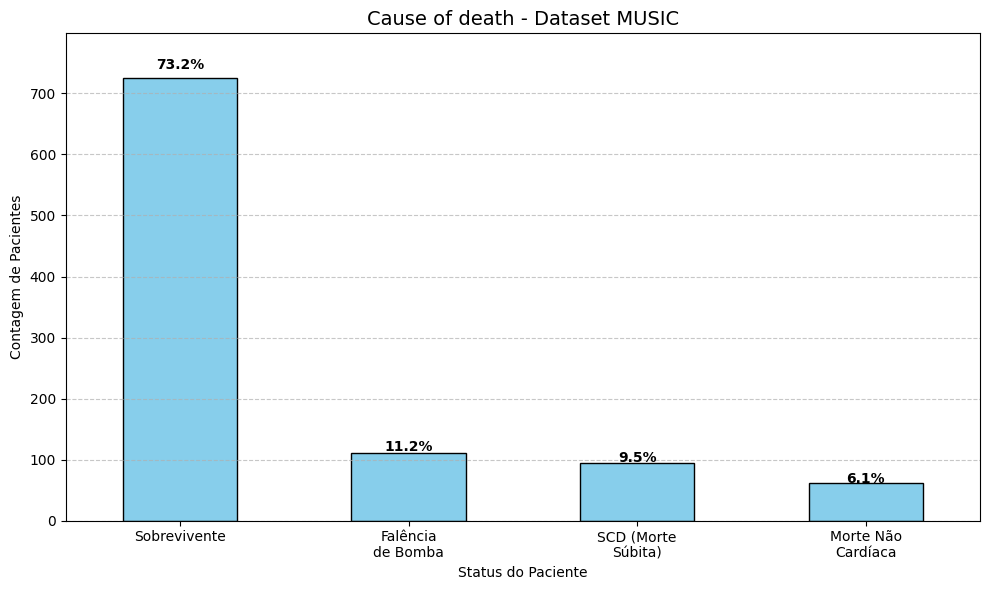
\includegraphics[width=16cm]{figuras/distribuicao_causa_da_morte}
    }{
        \Fonte{elaborado pelo autor (2026).}
    }
\end{figure}


Ao analisar a divisão dos dados, nota-se um desbalanceamento natural entre os pacientes vivos (tratados como dados censurados) e aqueles que sofreram o desfecho fatal. A predominância de pacientes vivos é comum, mas pode tornar mais desafiadora a tarefa de ensinar o modelo a identificar os padrões sutis no ECG relacionados à morte súbita cardíaca. No entanto, ao desconsiderarmos as mortes por outras causas — tratando-as também como censura — e focarmos estritamente nos eventos cardíacos, chegamos a um total de 205 pacientes, o que representa 20,67\% da base de dados. Do ponto de vista do treinamento de redes neurais, este é um cenário excelente. Muitos estudos na literatura médica lidam com um desbalanceamento muito mais severo, frequentemente operando com taxas de eventos na casa dos 10\% ou menos \cite{physionet2020cardiovascular}. Portanto, essa proporção de 20\% nos oferece uma quantidade de exemplos positivos bastante sólida para que o modelo consiga aprender de forma robusta. É um desafio desbaleamento, mas é um cenário muito mais favorável do que o encontrado em muitos outros estudos, o que aumenta as chances de desenvolver um modelo preditivo eficaz para a morte súbita cardíaca. Para resolver este desbalanceamento, existem diversas técnicas, a que irei utulizar é a Momentum Contrast (MOCO) \cite{he2020momentum} que ao adaptado ao modelo de sobrevivência, é uma técnica de aprendizado auto-supervisionado que pode ser utilizada para lidar com o desbalanceamento em conjuntos de dados. O MOCO é projetado para aprender representações robustas e discriminativas, mesmo quando há uma quantidade limitada de exemplos positivos (neste caso, pacientes que sofreram morte súbita cardíaca). Ele funciona criando um banco de memória que armazena representações de amostras anteriores, permitindo que o modelo aprenda a distinguir entre amostras positivas e negativas de forma eficaz. Ao utilizar o MOCO, é possível melhorar a capacidade do modelo de identificar padrões relevantes no ECG relacionados à morte súbita cardíaca, mesmo em um cenário desbalanceado.

Vou usar o subject-info.csv como gabarito antes de usar os sinais de ECG, ou seja, vou usar os dados clínicos e demográficos dos pacientes para treinar modelos com redes neurais comun e depois outros modelo com rede neural  mas complexa como Redes Neurais Convolucionais \gls{CNNs} usar os sinais de ECG nas \gls{CNNs} para comparar entre os modelos se com ECG os resultados são preciso e melhores ou não é tão relevante. Já os dados csv ja são suficiente para ter um bom resultado, menos custo computacional, e mais fácil de interpretar os resultados, já os sinais de ECG são mais complexos, exigem mais processamento e podem ser mais difíceis de interpretar os resultados, mas podem fornecer informações adicionais que não estão presentes nos dados clínicos e demográficos. Portanto, a escolha entre usar os dados clínicos e demográficos ou os sinais de ECG é dois pontos importante primeiro validação de hipotise, que os sinais de ECG pode encontrar padrões relacionados a morte súbita cardíaca, e segundo é o fato que os dados clínicos e demográficos são exames dificis de serem encontrados, em todos os pacientes pois são solicitado pelo medico apenas em casos mais graves, alem disso alguns são  exames caros ou complicado ao realizar, já os sinais de ECG são mais fáceis de serem encontrados, pois são exames mais comuns e baratos, e podem ser realizados em uma grande variedade de pacientes. Portanto, a escolha entre usar os dados clínicos e demográficos ou os sinais de ECG depende dos objetivos do estudo, dos recursos disponíveis e da viabilidade de obtenção dos dados.



\subsection{Grande volume dos sinais} \label{sec:grande_volume}

O grande volume de dados dos sinais de ECG Holter de 24 horas representa um desafio significativo para o processamento e análise. Cada paciente tem um registro contínuo de sinais de ECG ao longo de um período extenso, o que resulta em uma quantidade massiva de dados a ser processada. O processamento eficiente desses dados requer técnicas avançadas de pré-processamento, como filtragem, segmentação e extração de características relevantes. Além disso, o treinamento de modelos preditivos com esse volume de dados pode ser computacionalmente intensivo, exigindo recursos computacionais robustos e estratégias de otimização para garantir que o modelo possa aprender efetivamente a partir dos sinais sem sobrecarregar os sistemas de processamento. Estão registrado 992 paciente com três derivações de ECG Holter de 24 horas, com uma frequência de amostragem de 200 \gls{Hz}, o que resulta em um total de 17.280.000 pontos de dados por paciente (200 amostras por segundo x 60 segundos por minuto x 60 minutos por hora x 24 horas). Isso significa que, para os 992 pacientes, o volume total de dados de ECG Holter é de aproximadamente, treinar bilhões de pontos de dados (17.280.000 pontos por paciente x 992 pacientes), é inviavel processar e analisar esse volume de dados sem uma abordagem eficiente de pré-processamento e extração de características. Para lidar com esse desafio, técnicas de redução de dimensionalidade, como a utilização de redes neurais convolucionais para extrair características relevantes dos sinais, podem ser aplicadas para reduzir o volume de dados enquanto preservam as informações essenciais para a análise preditiva.

% \subsection{Exemplo de subseção} \label{sec:ex_sec}




%Testando o símbolo $\symE$

%\lipsum[5]  % Simulador de texto, ou seja, é um gerador de lero-lero.

%	\begin{alineas}
%		\item Lorem ipsum dolor sit amet, consectetur adipiscing elit. Nunc dictum sed tortor nec viverra.
%		\item Praesent vitae nulla varius, pulvinar quam at, dapibus nisi. Aenean in commodo tellus. Mauris molestie est sed justo malesuada, quis feugiat tellus venenatis.
%		\item Praesent quis erat eleifend, lacinia turpis in, tristique tellus. Nunc dictum sed tortor nec viverra.
%		\item Mauris facilisis odio eu ornare tempor. Nunc dictum sed tortor nec viverra.
%		\item Curabitur convallis odio at eros consequat pretium.
%	\end{alineas}



